\documentclass[12pt]{article}
\usepackage{graphicx}
\usepackage{caption}
\usepackage{subcaption}
\usepackage{tikz}
\usepackage{venndiagram}
\usepackage{tcolorbox}
\usepackage{listings}
\usepackage{enumitem}
\usepackage{amsmath}
\usepackage{amssymb}
\usepackage{colortbl}
\usepackage{xcolor}
\usepackage[margin=1cm, top=1.5cm, bottom=1.5cm]{geometry}
\usepackage{fancyhdr} % Paquete para encabezados y pies de página

\tcbuselibrary{breakable}

\title{\textbf{Álgebra Superior I\\
Tarea 02: Relaciones y Funciones}}
\author{Rendón Ávila Jesús Mateo}
\date{\today}

\pagestyle{fancy} % Establece el estilo de página como fancy
\fancyhf{} % Limpia cualquier configuración previa de encabezado y pie de página
\fancyhead[L]{Rendón Ávila Jesús Mateo} % Encabezado izquierdo
\fancyhead[R]{Tarea 02: Relaciones y Funciones} % Encabezado derecho
\fancyfoot[C]{\thepage} % Pie de página centrado con el número de página

\begin{document}

%\maketitle
%\begin{center}
%\vspace{3cm}
%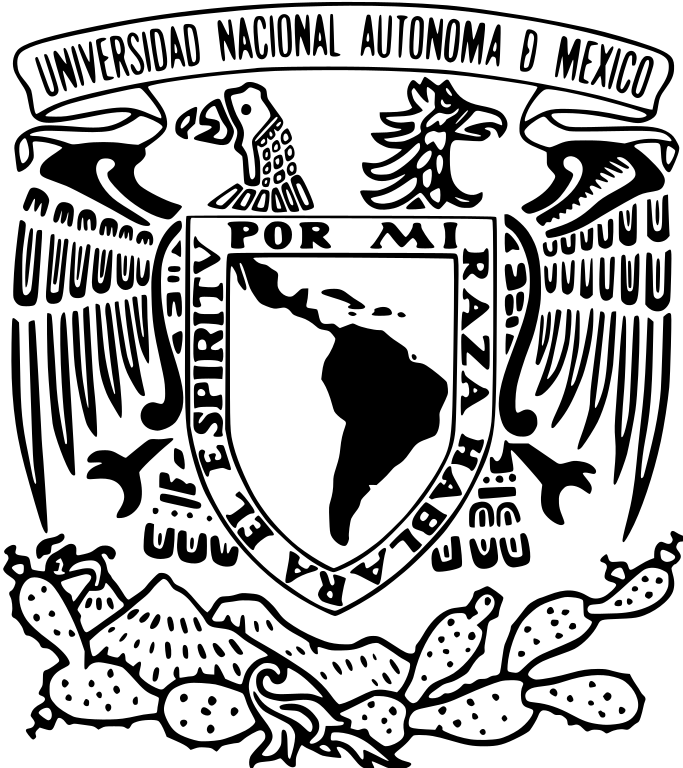
\includegraphics[width=0.195\textwidth]{Escudo.png}
%\hspace{0.5cm}
%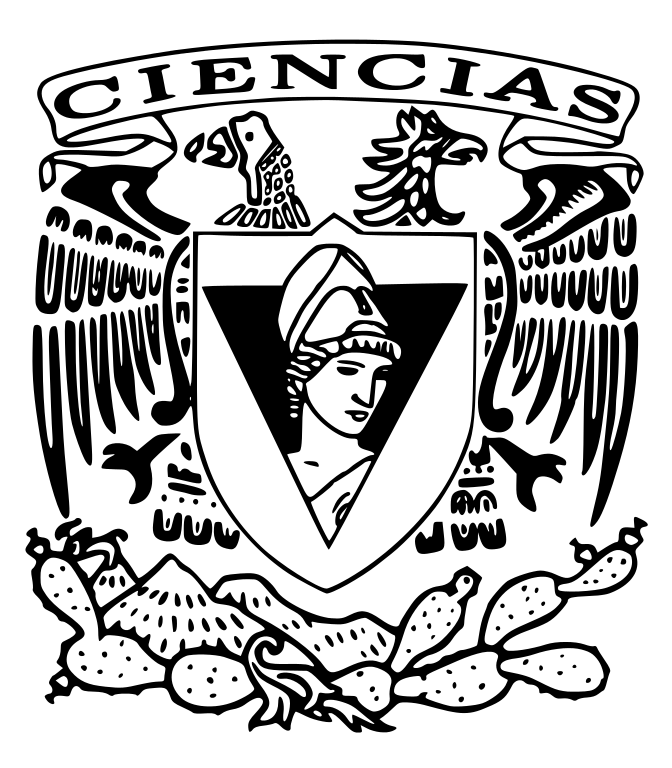
\includegraphics[width=0.203\textwidth]{logo_ciencias.png}
%\end{center}
%\begin{center}
%    \vspace{1cm}
%    \textbf{Universidad Nacional Autónoma de México}\\
%    Facultad de Ciencias\\
%    Profesora: Cristina Angélica Núñez Rodríguez\\
%\end{center}

%\newpage

%
% Ejercicio 1
%
$\bullet$ \textbf{1.} Determinar qué propiedades (reflexividad, simetría, antisimetría o transitividad) cumplen las siguientes
relaciones y determinar cuáles son una relación de equivalencia o de orden (parcial o total).

\begin{enumerate}[label=\alph*)]
    \item $R = \{(x,y) \in \mathbb{R} \times \mathbb{R} | x-y \textit{ es múltiplo de 3}\}$

    \textit{Reflexividad}. Como $0$ es múltiplo de cualquier número y ademas $\forall x \in \mathbb{R}$ se cumple que $x-x = 0$, entonces $R$ satisface reflexividad.\\

    \textit{Simetría}. Si $(x-y)$ es un múltiplo de $3$, entonces $(y-x)$ también será múltiplo de $3$, en particular el inverso de $(x,y)$. De lo
    anterior decimos que $R$ satisface la simetría.\\

    \textit{Antisimetría}. La antisimetría no se cumple en $R$, basta dar el contraejemplo $(3,6)$ y $(6,3)$ donde $3 \neq 6$.\\

    \textit{Transitividad}. Finalmente, la relación satisface la transitividad pues $\forall$ $(x-y), (y-z)$ que es múltiplo de $3$, también el número $(x-z)$ satisface
    el ser múltiplo de 3.\\

    Por lo tanto $R$ es de equivalencia.

    \item $R = \{(1,1),(2,2),(1,2),(2,1),(3,3),(3,4),(4,3),(4,4)\}$, donde $A = \{1,2,3,4\}$

    \textit{Reflexividad}. Como $\forall x \in A, \text{ } \exists (x,x) \in R$ decimos que R es reflexiva.\\ 

    \textit{Simetría}. Como $(1,2), (3,4) \in R$  y $(2,1), (4,3) \in R$ entonces R es simétrica, para los pares $(x,x)$ la simetría es por
    vacuidad.\\

    \textit{Antisimetría}. No se satisface.

    \textit{Transitividad}. 
    \begin{align*}
        (1,1), (1,2)&\sim (1,2)\\
        (2,2), (2,1)&\sim (2,1)\\
        (1,2), (2,1)&\sim (1,1)\\
        (2,1), (1,2)&\sim (2,2)\\
    \end{align*}
    Para el caso de $3$ y $4$ es similar, así $R$ es transitiva.\\
    
    Por lo tanto $R$ es de equivalencia.

    \item $R = \{(1,1),(2,2),(3,3),(4,4),(1,2),(1,3),(1,4),(2,3)\}$, donde $A = \{1,2,3,4\}$

    \textit{Reflexividad}. Como $\forall x \in A, \text{ } \exists (x,x) \in R$ decimos que R es reflexiva.\\ 

    \textit{Simetría}. Como $(1,2) \in R$  y $(2,1) \notin R$, entonces R no es simétrica.\\

    \textit{Antisimetría}. No se satisface.

    \textit{Transitividad}. El caso trascendente es que $\exists (1,2), (2,3) \in R$ y también $(1,3) \in R$\\

    Por lo tanto R no es de equivalencia.\\

    \item La relación en $A = \mathbb{R}$ definida por $a \sim b \Longleftrightarrow a \leq b$\\

    Por definición de $\leq$ entonces todo numero es igual a si mismo por lo que $(a,a) \in R$, lo que hace a $R$ reflexiva.\\
    
    como no puede ser $a \sim b$, si $a$ menor que $b$, que pase $b \sim a$ por lo que $R$ no es simétrica.\\

    $R$ es una relación que cumple antisimetría pues si $x \leq y$ y $y \leq x$ entonces $x = y$.\\

    También por definición de $\leq$ satisface la transitividad.\\

    Sim embargo al no haber mínimos ni cotas en $\mathbb{R}$ no podemos hablar de un orden total.

    \item La relación en $A = P(X)$ definida por $A \sim B \Longleftrightarrow A \subseteq B$

    Como todo conjunto esta contenido en si mismo entonces $A \sim A$, por lo que $R$ es reflexiva.\\

    Sin embargo la simetría no se cumple pues si $A \subseteq B$ no necesariamente $B \subseteq A$.\\

    La antisimetría se cumple de manera similar al problema anterior, pues si  $A \subseteq B$ y $B \subseteq A$ entonces $A = B$.\\

    Lo mismo ocurre con la transitividad pues si $A \subseteq B$ y $B \subseteq C$ entonces $A \subseteq C$.

    Ademas hay un mínimo que es el conjunto $\varnothing$, por lo que estamos en un orden parcial.
\end{enumerate}

\vspace{0.5cm}
%
% Ejercicio 2
%
$\bullet$ \textbf{2.} Demostrar que la siguiente relación es de equivalencia e indicar quién es el conjunto cociente asociado. 
Sea $A = \{(a, b) \mid a, b \in \mathbb{Z}, b \neq 0\}$ y $R$ la relación definida en $A$ tal que $(a, b) \sim (c, d)$ si y sólo si $ad = bc$.\\

$P.d$ $R$ es reflexiva, simétrica y transitiva.\\

\textit{R es reflexiva.}\\

$\forall (a, b) \in A$ se debe satisfacer que $(a, b) \sim (a, b)$
\begin{align*}
    (a, b) &\sim (a, b)\\
    ab &= ba \textit{ (por conmutación en ba)}\\
    ab &= ab
\end{align*}
Así, decimos que $R$ es reflexiva.\\

\textit{R es simétrica.}\\

Si $(a, b) \sim (c, d)$ entonces se deberá satisfacer que $(c, d) \sim (a, b)$

\begin{align*}
    (a, b) &\sim (c, d)\\
    ad &= cb \\
    cb &= ad \textit{ (por conmutación en ad)}\\ 
    cb &= da\\
    (c, d) &\sim (a, b)
\end{align*}
Así, $R$ es simétrica.\\

\textit{R es transitiva.}\\

Si $(a, b) \sim (c, d)$ y $(c, d) \sim (e, f)$ entonces se deberá satisfacer que $(a, b) \sim (e, f)$
\begin{align*}
    (a, b) &\sim (c, d)\\
    ad &= bc\\
    \\
    (c, d) &\sim (e, f)\\
    cf &= de\\
\end{align*}
Por propiedades de los $\mathbb{Z}$
\begin{align*}
    ad \bullet cf &= bc \bullet de \textit{ (por cancelación del producto en $\mathbb{Z}$)}\\
    af &= be\\
    (a, b) &\sim (e, f)
\end{align*}
Así concluimos que $f$ es transitiva.\\
\\
$\therefore$ $R$ es de equivalencia $_\blacksquare$\\

El conjunto cociente asociado es $A / R = \{[(a, b)]_R \mid (a, b) \in A\}$, por la definición  de la relación entonces:\\
\begin{center}
    $A / R = \{\{(c, d)\} \mid (a, b) \in A \textit{ y } ad = bc\}$
\end{center}
Por lo anterior podemos decir que los elementos de $A / R$ son los $\mathbb{Q}$.


\vspace{0.5cm}
%
% Ejercicio 3
%
$\bullet$ \textbf{3.} Diga cuál de las siguientes relaciones son funciones (justifica tu respuesta):
\begin{enumerate}[label=\alph*)]
    \item $R \subseteq \{1,2,3\} \times \{1,2,3\}$ definida como:\\
    \begin{center}
        $R = \{(1,2),(2,2),(3,3),(2,3),(1,1)\}$
    \end{center}
    No es función pues $1$ está relacionado con $1$ y $2$ y también $2$ está relacionada con $2$ y $3$.

    \item $S \subseteq \mathbb{N} \times \mathbb{N}$ definida como:\\
    \begin{center}
        $S = \{(n,m) \mid n < m\}$
    \end{center}
    Es fácil ver que si $n$ está en el dominio de $S$ y $n = 1$, entonces para cualquier $m > 1$ en el codominio tendremos que $n = 1$
    va a satisfacer el estar relacionado con $m > 1$, con lo que $S$ no es función.
    
    \item $T \subseteq ( \mathbb{Z} \times \mathbb{Z} ) \times \mathbb{Z}$ definida como:\\
    \begin{center}
        $T = \{((n,m),n+m) \mid n, m \in \mathbb{Z}\}$
    \end{center}
    Como no puede ser que $m \neq m$ o $n \neq n$, el valor para $n + m$ debe ser único.\\

    Pensemos en una $m'$ que satisfaga $n + m = n + m'$
    \begin{align*}
        n + m &= n + m'\\
        m &= m'
    \end{align*}
    Lo mismo ocurre con una $n'$ por lo que $n + m$ es un valor único.\\

    $\therefore$ $f$ es función pues $n + m$ es un valor único para cualquier $n, m \in \mathbb{Z}$.

\end{enumerate}

\vspace{0.5cm}
%
% Ejercicio 4
%
$\bullet$ \textbf{4.} Sea ${\displaystyle f: \mathbb{Q} \longrightarrow \mathbb{Z}}$, con regla de correspondencia:\\
\begin{center}
    ${\displaystyle f\left(\frac{a}{b}\right) = a}$
\end{center}
Para toda $a.b \in \mathbb{Z}$, con $b \neq 0$. ¿Será que ${\displaystyle f}$ está bien definida?. Justifica tu respuesta.\\

Como en $\mathbb{Q}$ se tiene que $\frac{1}{2} = \frac{2}{4} = \frac{3}{6}$, si aplicamos la regla de correspondencia:\\

\begin{align*}
    f\left(\frac{1}{2}\right) &= 1\\
    f\left(\frac{2}{4}\right) &= 2\\
    f\left(\frac{3}{6}\right) &= 3\\
\end{align*}
Como $f\left(\frac{1}{2}\right) \neq f\left(\frac{2}{4}\right) \neq f\left(\frac{3}{6}\right)$ y ademas $\frac{1}{2} = \frac{2}{4} = \frac{3}{6}$
podemos decir que:
\begin{align*}
    f\left(\frac{1}{2}\right) &= 1\\
    f\left(\frac{1}{2}\right) &= 2\\
    f\left(\frac{1}{2}\right) &= 3\\
\end{align*}
De lo anterior decimos que $f$ no está bien definida.

\vspace{0.5cm}
%
% Ejercicio 5
%
$\bullet$ \textbf{5.} Sea ${\displaystyle f: A \longrightarrow B}$ y sean $Y_1, Y_2 \subseteq B$. Demuestra lo siguiente:\\

    Para este ejercicio vamos a fijar la siguiente definición:
    \begin{tcolorbox}[title=\textbf{Definiciones}, colback=blue!15!white, colframe=black!, breakable]
        $Def$. Sean $f: A \longrightarrow B$ y $X \subseteq A$\\
        La \textbf{imagen directa} de $X$ bajo $f$ es el conjunto:
        \begin{center}
            $f[X] = \{y \in B \mid \exists x \in X \textit{ tal que } f(x) = y\}$
        \end{center}
        $Def$. Sean $f: A \longrightarrow B$ y $Y \subseteq B$\\
        La \textbf{imagen inversa} de $Y$ bajo $f$ es el conjunto:
        \begin{center}
            $f^{-1}[Y] = \{x \in A \mid \exists y \in Y \textit{ tal que } f(x) = y\}$
        \end{center}    
    \end{tcolorbox}

\begin{enumerate}[label=\alph*)]
    \item ${ f^{-1}} [\varnothing] = \varnothing$\\

    Sea $x \in f^{-1}[\varnothing]$, por definición de imagen inversa, existe $y \in \varnothing$ tal que 
    \begin{center}
        $f(x) = y$ \textbf{!}\\
    \end{center}
    Como no puede ser $y \in \varnothing$, entonces $f^{-1}[\varnothing] = \varnothing$ $_\blacksquare$

    \item $f^{-1} [Y_1 \cup Y_2] =  f^{-1}[Y_1] \cup f^{-1}[Y_2]$\\

    $\subseteq$) $ f^{-1} [Y_1 \cup Y_2] \subseteq  f^{-1}[Y_1] \cup  f^{-1}[Y_2]$\\

    Sea $x \in f^{-1} [Y_1 \cup Y_2]$, por definición imagen inversa, entonces existe $y \in Y_1 \cup Y_2$ tal que:
    \begin{center}
        $f(x) = y$\\
    \end{center}
    Por definición de unión, si $y \in Y_1 \cup Y_2$, entonces $y \in Y_1$ o $y \in Y_2$\\

    Caso $y \in Y_1$. Como existe $y \in Y_1$ de forma que $f(x) = y$, por definición de imagen inversa concluimos que:
    \begin{center}
        $x \in f^{-1}[Y_1]$
    \end{center}
    Caso $y \in Y_2$. Como existe $y \in Y_2$ de forma que $f(x) = y$, por definición de imagen inversa concluimos que:
    \begin{center}
        $x \in f^{-1}[Y_2]$
    \end{center}
    Así podemos decir que $x \in f^{-1}[Y_1] \cup f^{-1}[Y_2]$\\

    $\therefore f^{-1} [Y_1 \cup Y_2] \subseteq  f^{-1}[Y_1] \cup  f^{-1}[Y_2]$\\

    $\supseteq$) $f^{-1}[Y_1] \cup f^{-1}[Y_2] \subseteq f^{-1} [Y_1 \cup Y_2]$\\

    Sea $x \in f^{-1}[Y_1] \cup f^{-1}[Y_2]$, por definición de unión
    \begin{center}
        $x \in f^{-1}[Y_1]$ o $x \in f^{-1}[Y_2]$
    \end{center}
    Si $x \in f^{-1}[Y_1]$, por definición de imagen inversa, entonces existe $y \in Y_1$ tal que $f(x) = y$\\

    Si $x \in f^{-1}[Y_2]$, por definición de imagen inversa, entonces existe $y \in Y_2$ tal que $f(x) = y$\\

    como $y \in Y_1$ o $y \in Y_2$, entonces $y \in Y_1 \cup Y_2$ de forma que $f(x) = y$, por definición de imagen inversa concluimos que:
    \begin{center}
        $x \in f^{-1}[Y_1 \cup Y_2]$
    \end{center}
    Así $f^{-1}[Y_1] \cup f^{-1}[Y_2] \subseteq f^{-1} [Y_1 \cup Y_2]$\\

    $\therefore f^{-1} [Y_1 \cup Y_2] =  f^{-1}[Y_1] \cup f^{-1}[Y_2]$ $_\blacksquare$

    \item ${\displaystyle f^{-1}} [Y_1 \cap Y_2] = {\displaystyle f^{-1}}[Y_1] \cap {\displaystyle f^{-1}}[Y_2]$\\

    $\subseteq$) $f^{-1} [Y_1 \cap Y_2] \subseteq  f^{-1}[Y_1] \cap f^{-1}[Y_2]$\\

    Sea $x \in f^{-1} [Y_1 \cap Y_2]$, por definición de imagen inversa, existe $y \in Y_1 \cap Y_2$ tal que
    \begin{center}
        $f(x) = y$
    \end{center}
    Por definición de intersección, $y \in Y_1$ y $y \in Y_2$.\\

    Por $y \in Y_1$ de forma que $f(x) = y$, entonces $x \in f^{-1}[Y_1]$.\\

    Por $y \in Y_2$ de forma que $f(x) = y$, entonces $x \in f^{-1}[Y_2]$.\\

    Como  $x \in f^{-1}[Y_1]$ y $x \in f^{-1}[Y_2]$, entonces $x \in f^{-1}[Y_1] \cap f^{-1}[Y_2]$\\

    $\therefore f^{-1} [Y_1 \cap Y_2] \subseteq  f^{-1}[Y_1] \cap f^{-1}[Y_2]$\\

    $\supseteq$)  $f^{-1}[Y_1] \cap f^{-1}[Y_2] \subseteq f^{-1} [Y_1 \cap Y_2]$\\

    Sea $x \in f^{-1}[Y_1] \cap f^{-1}[Y_2]$, por definición de intersección:
    \begin{center}
        $x \in f^{-1}[Y_1]$ y $x \in f^{-1}[Y_2]$
    \end{center}
    Por  $x \in f^{-1}[Y_1]$ de forma que $f(x) = y$, por definición de imagen inversa existe $y \in Y_1$\\

    Por  $x \in f^{-1}[Y_2]$ de forma que $f(x) = y$, por definición de imagen inversa existe $y \in Y_2$\\

    Así $y \in Y_1 \cap Y_2$, como $f(x) = y$, entonces $x \in f^{-1}[Y_1 \cap Y_2]$\\

    $\therefore f^{-1}[Y_1] \cap f^{-1}[Y_2] \subseteq f^{-1} [Y_1 \cap Y_2]$\\

    $\therefore {\displaystyle f^{-1}} [Y_1 \cap Y_2] = {\displaystyle f^{-1}}[Y_1] \cap {\displaystyle f^{-1}}[Y_2]$ $_\blacksquare$

    \item $f^{-1} [B] \backslash  f^{-1} [Y_1] = f^{-1}[B \backslash Y_1]$\\

    $\subseteq$) $f^{-1} [B] \backslash  f^{-1} [Y_1] \subseteq f^{-1}[B \backslash Y_1]$\\

    Sea $x \in f^{-1} [B] \backslash  f^{-1} [Y_1]$ por definición de imagen inversa, existe $y \in f^{-1} [B] \backslash  f^{-1} [Y_1]$ tal que $f(x) = y$\\

    Por definición de diferencia, entonces $x \in f^{-1} [B]$ y $x \notin f^{-1} [Y_1]$. Así, de nuevo por definición de imagen inversa tenemos que:\\

    Como $x \in f^{-1} [B]$, entonces existe $y \in B$ tal que $f(x) = y$.\\

    Como $x \notin f^{-1} [Y_1]$, entonces  $f(x) \neq y$.\\

    De lo anterior podemos afirmar que $y \in B \backslash Y_1$ de forma que $f(x) = y$, por definición de imagen inversa, entonces:
    \begin{center}
        $x \in f^{-1}[B \backslash Y_1]$
    \end{center}
    Así $f^{-1} [B] \backslash  f^{-1} [Y_1] \subseteq f^{-1}[B \backslash Y_1]$\\

    $\supseteq$) $f^{-1}[B \backslash Y_1] \subseteq f^{-1} [B] \backslash  f^{-1} [Y_1]$\\

    Sea $x \in  f^{-1}[B \backslash Y_1]$, por definición de imagen inversa, entonces existe $y \in B \backslash Y_1$ tal que $f(x) = y$.\\

    Por definición de diferencia:
    \begin{center}
        $y \in B$, y\\
        $y \notin Y_1$
    \end{center}
    Como $y \in B$ de forma que $f(x) = y$, entonces $x \in f^{-1}[B]$.\\

    Como $y \notin Y_1$, entonces$f(x) \neq y$ de forma que  $x \notin f^{-1}[Y_1]$.\\

    De lo anterior podemos decir que $x \in f^{-1}[B] \backslash f^{-1}[B]$.\\

    $\therefore f^{-1}[B \backslash Y_1] \subseteq f^{-1} [B] \backslash  f^{-1} [Y_1]$

    $\therefore f^{-1} [B] \backslash  f^{-1} [Y_1] = f^{-1}[B \backslash Y_1]$. $_\blacksquare$

\end{enumerate}

\vspace{0.5cm}
%
% Ejercicio 6 
%
$\bullet$ \textbf{6.} Da un contraejemplo de una función ${\displaystyle f: A \longrightarrow B}$ y $X_1, X_2 \subseteq A$ tales que:
\begin{center}
    ${\displaystyle f} [X_1 \cap X_2] \neq {\displaystyle f}[X_1] \cap {\displaystyle f}[X_2]$
\end{center}
Sea $A = \{1,2,3,4\}$ y $B=\{1,4,9,16\}$. Si $f: A \longrightarrow B$ con regla $f(a) = a^2$.\\

digamos que $X_1 = \{2,3,4\}$ y $X_2 =\{1,2,3\}$, la intersección $X_1 \cap X_2 = \{2,3\}$.\\

Las imágenes directas de los conjuntos anteriores son:
\begin{center}
    $f[X_1] = \{4, 9, 16\}$\\

    $f[X_2] = \{1, 4, 9\}$ 
\end{center}
Entonces $f[X_1 \cap X_2] =\{4, 9\}$.\\

Si hacemos la intersección de $f[X_1] = \{4, 9, 16\}$ con $f[X_2] = \{1, 4, 9\}$, tendremos que:
\begin{center}
    $f[X_1] \cap f[X_2] = \{4, 9\}$\\
\end{center}
De lo anterior vemos que $f[X_1 \cap X_2] = f[X_1] \cap f[X_2] = \{4, 9\}$. Por lo que hemos dado un contraejemplo valido 
que contradice la no igualdad dada.

\vspace{0.5cm}
%
% Ejercicio 7
%
$\bullet$ \textbf{7.} Sean ${\displaystyle f: A \longrightarrow B}$ y ${\displaystyle g: B \longrightarrow C}$ funciones. Demuestre lo siguiente:
\begin{enumerate}[label=\alph*)]
    \item si ${\displaystyle f}$ y ${\displaystyle g}$ son inyectivas, entonces ${\displaystyle g \circ f}$ es inyectiva\\

    Sea $x_1$ y $x_2$ de forma que:

    \begin{center}
        $(g \circ f) (x_1) = g(f(x_1)) = g(f(x_2)) = (g \circ f) (x_1)$\\
    \end{center}
    como $g$ es inyectiva, entonces:

    \begin{center}
        $f(x_1) = f(x_2)$\\
    \end{center}
    Como $f$ es inyectiva, entonces:

    \begin{center}
        $x_1 = x_2$\\
    \end{center}
    $\therefore g \circ f$ es inyectiva $_\blacksquare$\\

    \item si ${\displaystyle f}$ y ${\displaystyle g}$ son sobreyectivas, entonces ${\displaystyle g \circ f}$ es sobreyectiva\\

    sea $z \in C$ cualquiera, entonces por ser $g$ suprayectiva:
    \begin{center}
        $\exists y \in B$ tal que\\

        $g(y) = z$
    \end{center}
    También, sea $y \in B$ cualquiera, entonces por ser $f$ suprayectiva:
    \begin{center}
        $\exists x \in A$ tal que\\

        $f(x) = y$
    \end{center}

    por igualdad de $f(x) = y$, entonces 
    \begin{center}
        $(g \circ f) (x) = g(f(x)) = g(y) = z$
    \end{center}
    Así $g \circ f$ es suprayectiva. $_\blacksquare$\\

    \item si ${\displaystyle f}$ y ${\displaystyle g}$ son biyectivas, entonces ${\displaystyle g \circ f}$ es biyectiva.\\

    Para probar que $g \circ f$ es biyectiva, hay que probar que es inyectiva y sobreyectiva, lo cual se ha hecho en los dos incisos anteriores 
    considerando $f$ y $g$ inyectivas y suprayectivas.\\

    Así $g \circ f$ es biyectiva $_\blacksquare$
\end{enumerate}

\vspace{0.5cm}
%
% Ejercicio 8
%
$\bullet$ \textbf{8.} Sean ${\displaystyle f: A \longrightarrow B}$ y ${\displaystyle g: B \longrightarrow C}$ funciones invertibles.
\begin{enumerate}[label=\alph*)]
    \item Demuestre que ${\displaystyle g \circ f}$ es invertible\\

    Para esta demostración vamos a fijar la siguiente definición:

    \begin{tcolorbox}[title=\textbf{Definiciones}, colback=blue!15!white, colframe=black!, breakable]

    $Def$. Sea $f$ una función tal que $f: A \longrightarrow B$, diremos que $f$ es invertible si existe una función 
    $g: B \longrightarrow A$ que satisface:
\begin{center}
    $g \circ f = 1_A$ y\\

    $f \circ g = 1_b$ 
\end{center}

    denotaremos por $f^{-1}$ a dicha función $g$, y le llamaremos la función inversa de $f$.
    \end{tcolorbox}

    Como $f$ es invertible, enotnces existe $f^{-1}$ tal que satisface:
    \begin{center}
        $f^{-1} \circ f = 1_A$ y\\
         $f \circ f^{-1} = 1_B$
    \end{center}
    De igual forma, como $g$ es invertible, enotnces existe $g^{-1}$ tal que satisface:
    \begin{center}
        $g^{-1} \circ g = 1_B$ y\\
         $g \circ g^{-1} = 1_C$
    \end{center}
    $P.d$. Hay que exhibir una funcíon $h$ que satisfaga: 
    \begin{center}
        $h \circ (g \circ f) = 1_A$ y\\
         $(g \circ f) \circ h = 1_C$
    \end{center}
    Sabemos que $g \circ f: A \longrightarrow C$, por lo que debe ser $h: C \longrightarrow A$.\\

    Cómo $f$ y $g$ son invertibles enotnces $f^{-1}: B \longrightarrow A$ y $g^{-1}: C \longrightarrow B$, así propongamos:
    \begin{center}
        $h = f^{-1} \circ g^{-1}$
    \end{center}
    De lo anterior $h: C \longrightarrow A$.\\

    Por $f$ sabemos que $f(x) = y$ y por ser invertible, entonces $f^{-1}(y) = x$.\\

    Para $g$ sabemos que $g(y) = z$ y por ser invertible, entonces $g^{-1}(z) = y$.\\

    Como ya sabemos que efectivamente $f^{-1}$ y $g^{-1}$ son inversas de $f$ y $g$, vamos a hacer la composición $h \circ (g \circ f)$, usando 
    la propuesta que hicimos par $h$:
    \begin{align*}
        (h \circ (g \circ f))(x) &= h((g \circ f)(x))\\
        h((g \circ f)(x)) &= h(g(f(x)))\\
        h(g(f(x))) &= h(g(y))\\
        h(g(y)) &= h(z)
    \end{align*}

    vamos a probar que $h(z) = x$ usando las inversas que ya mostramos para $f$ y $g$ usando a $h$:\\

    Como $h = f^{-1} \circ g^{-1}$, entonces:
    \begin{align*}
        (f^{-1} \circ g^{-1})(z) &= f^{-1}(g^{-1}(z))\\
        f^{-1}(g^{-1}(z)) &= f^{-1}(y)\\
        f^{-1}(y) &= x
    \end{align*}
    Como h(z) = x, entonces $h$ es inversa izquierda de $g \circ f$.\\

    Ahora veremos que $h$ cumpla con:
    \begin{center}
        $(g \circ f) \circ h = z$
    \end{center}
    Como sabemos que $f^{-1}$ y $g^{-1}$ son inversas de $f$ y $g$, vamos a hacer la composición de $(g \circ f) \circ h = z$:
    \begin{align*}
        ((g \circ f) \circ h)(z) &= (g \circ f)(h(z))\\
        (g \circ f)(h(z)) &= (g \circ f)(x)\\
        (g \circ f)(x) &= g(f(x))\\
        g(f(x)) &= g(y)\\
        g(y) &= z
    \end{align*}
    Como $(g \circ f) \circ h = z$, entonces $h$ es inversa izquierda de $g \circ f$.\\

    Así podemos decir que $h = (g \circ f)^{-1}$

    $\therefore g \circ f$ es invertible $_\blacksquare$

    \item Demuestre que ${\displaystyle (g \circ f)^{-1}} = {\displaystyle f^{-1} \circ g^{-1}}$\\

    Retomando lo que probamos en el inciso anterior, sabemos que $(g \circ f)^{-1} = h = f^{-1} \circ g^{-1}$.\\

    Pero vamos a desarrollar mas para no vernos tan flojos.\\

    Como $g \circ f: A \longrightarrow C$, sabemos que $(g \circ f)^{-1}: C \longrightarrow A$
    \begin{align*}
        (g \circ f)^{-1}(z) &= x
    \end{align*}
    Ahora, vamos a ver la composición $f^{-1} \circ g^{-1}$, usando lo obtenido en el inciso anterior:
    \begin{align*}
        f^{-1} \circ g^{-1}(z) &= f^{-1}(g^{-1}(z))\\
        f^{-1}(g^{-1}(z)) &= f^{-1}(y)\\
        f^{-1}(y) &= x 
    \end{align*}
    De lo anterior vemos que se cumple la igualdad $(g \circ f)^{-1} = h = f^{-1} \circ g^{-1}$.\\

    $\therefore$ $(g \circ f)^{-1} = f^{-1} \circ g^{-1}$ $_\blacksquare$
    
\end{enumerate}

\vspace{0.5cm}
% 
% Ejercicio 9
%
$\bullet$ \textbf{9.} Sea ${\displaystyle f: A \longrightarrow B}$ inyectiva. Demostrar que si $B$ es finito entonces $A$ es finito y $\# A \leq \#B$\\

$P.d$. $A$ es un conjunto finito y $\# A \leq \#B$.\\

Como $f$ es una función inyectiva, entonces $\forall x_1, x_2 \in A$ si $f(x_1) = f(x_2)$ afirmamos que $x_1 = x_2$.\\

También por ser $B$ finito, entonces $\# B = n$, con $n \in \mathbb{N} - \{0\}$.\\

Por ser $f$ función decimos que $Dom(f) = A$ y ademas $Im(f) \subseteq B$.\\

De lo anterior
\begin{align*}
    \# Dom(f) &= \# A \text{ y}\\
    \# Im(f) &\leq \# B\\
\end{align*}
Por inyectividad tenemos que $\# Im(f) = \# Dom(f)$.\\
\\
Así $\# A \leq \# B$ $_\blacksquare$

\vspace{0.5cm}
%
% ejercicio 10
%
$\bullet$ \textbf{10.} Sea ${\displaystyle f: A \longrightarrow B}$ suprayectiva. Demostrar que si $A$ es finito entonces $B$ es finito y $\# B \leq \#A$\\

$P.d$. $B$ es un conjunto finito y $\# A \leq \#B$.\\

Como $f$ es una función biyectiva, entonces $\forall b \in B$, $\exists a \in A$ tal que $f(a) = b$, $i.e$ $Im(f) = B$\\

también por ser $A$ finito, entonces $\# A = n$, con $n \in \mathbb{N} - \{0\}$.\\

Por ser $f$ función decimos que $Dom(f) = A$, así el dominio es finito, ademas sabemos que $\# Im(f) \leq \# Dom(f)$.\\

De lo anterior
\begin{align*}
    \# Dom(f) &= \# A \text{ y}\\
    \# Im(f) &= \# B \text{ y}\\
    \# Im(f) &\leq \# Dom(f)\\
    \# B &\leq \# A
\end{align*}
Así queda demostrado que si ${\displaystyle f: A \longrightarrow B}$  es una función suprayectiva y $A$ es finito, entonces $B$ es finito y $\#B \leq \# A$ $_\blacksquare$

\end{document}